\chapter{Proverb 30}

\begin{figure}
  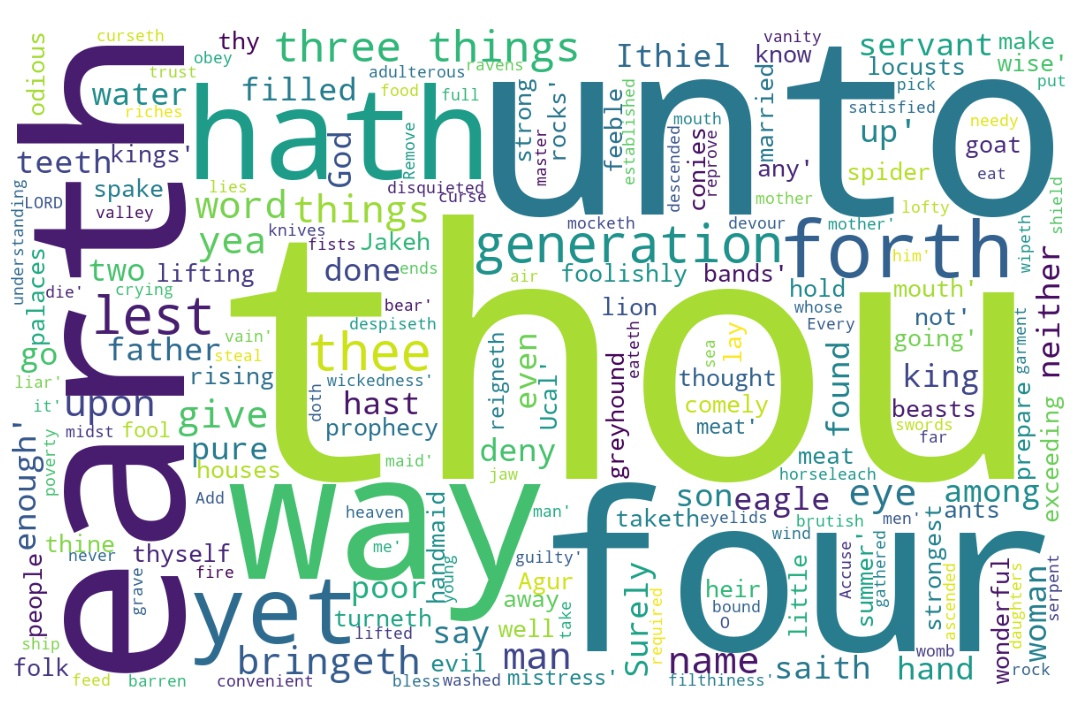
\includegraphics[width=\linewidth]{20OT-Proverbs/Proverb30-WordCloud.jpg}
  \caption{Proverb 30 Word Cloud}
  \label{fig:Proverb 30 word Cloud}
\end{figure}


\marginpar{\scriptsize \centering \fcolorbox{bone}{lime}{\textbf{A CONVERT TO WISDOM}}\\ (Proverb 30:1--33) 
\begin{compactenum}[I.][8]
    \item \textbf{Responds to Revealed Truth} \index[scripture]{Proverbs!Pro 30:01}(Pro 30:1)
    \item \textbf{Realizes his Brutish Condition} \index[scripture]{Proverbs!Pro 30:02-03}(Pro 30:2-3)
    \item \textbf{Respects God's Word} \index[scripture]{Proverbs!Pro 30:04-06}(Pro 30:4-6)
    \item \textbf{Requests Security from God} \index[scripture]{Proverbs!Pro 30:07-09}(Pro 30:7-9)
    \item Is \textbf{Repulsed by Wickedness} \index[scripture]{Proverbs!Pro 30:10-14}(Pro 30:10-14)
    \item \textbf{Recognizes Truth in Nature} \index[scripture]{Proverbs!Pro 30:15-31}(Pro 30:15-31)
    \item \textbf{Repents of Self-Promotion} \index[scripture]{Proverbs!Pro 30:32}(Pro 30:32)
\end{compactenum} }


\marginpar{\scriptsize \centering \fcolorbox{bone}{yellow}{\textbf{SEEING THE ASCENDANT ONE}}\\ (Proverb 30:1--33) 
\begin{compactenum}[I.][8]
    \item Who is \textbf{Listening} \index[scripture]{Proverbs!Pro 30:04}(Pro 30:4)
    \item Who is \textbf{Longing for Satisfaction} \index[scripture]{Proverbs!Pro 30:04}(Pro 30:4)
    \item Who is \textbf{Looking through Scripture} \index[scripture]{Proverbs!Pro 30:04}(Pro 30:4, \index[scripture]{Psalms!Psa 040:07}Psa 40:7)
    \item Who is \textbf{Laboring for Salvation} \index[scripture]{Proverbs!Pro 30:04}(Pro 30:4) -- only to find that he cannot succeed
    \item Who is \textbf{Lamenting Sin} \index[scripture]{Proverbs!Pro 30:04}(Pro 30:4) -- only to find that he cannot succeed
    \item Who is \textbf{Lost and Seeking} \index[scripture]{Proverbs!Pro 30:04}(Pro 30:4) 
    \item Who is \textbf{Lowly and Sorrowful} \index[scripture]{Proverbs!Pro 30:04}(Pro 30:4) 
\end{compactenum} }

\footnote{\textcolor[cmyk]{0.99998,1,0,0}{\hyperlink{TOC}{Return to end of Table of Contents.}}}\footnote{\href{https://www.audioverse.org/english/audiobibles/books/ENGKJV/O/Prov/1}{\textcolor[cmyk]{0.99998,1,0,0}{Proverbs Audio}}}\textcolor[cmyk]{0.99998,1,0,0}{The words of Agur the son of Jakeh, \emph{even} the \fcolorbox{bone}{lime}{prophecy}: the man spake unto Ithiel, even unto Ithiel and Ucal,}
[2] \textcolor[cmyk]{0.99998,1,0,0}{Surely I \emph{am} more \fcolorbox{bone}{lime}{brutish} than \emph{any} man, and have not the \fcolorbox{bone}{MYGOLD}{understanding} of a man.}\footnote{\textbf{Psalm 92:5-6} - O LORD, how great are thy works! and thy thoughts are very deep. [6] A brutish man knoweth not; neither doth a fool understand this.}
[3] \textcolor[cmyk]{0.99998,1,0,0}{I neither learned wisdom, nor have the knowledge of the holy.}
[4] \textcolor[cmyk]{0.99998,1,0,0}{Who hath ascended up into heaven, or descended? who hath gathered the wind in his fists? who hath bound the waters in a garment? who hath established all the ends of the earth? what \emph{is} his name, and what \emph{is} his son's name, if thou canst tell?}\footnote{\textbf{Exodus 3:13} - And Moses said unto God, Behold, when I come unto the children of Israel, and shall say unto them, The God of your fathers hath sent me unto you; and they shall say to me, What is his name? what shall I say unto them?}\footnote{\textbf{Job 26:8} - He bindeth up the waters in his thick clouds; and the cloud is not rent under them.}\footnote{\textbf{Job 38:37} - Who can number the clouds in wisdom? or who can stay the bottles of heaven,}\footnote{The connection is to the great KJV biblical truth of the Great Deep, starting back in Genesis.. The verse speaks to cosmology, or the structure of the universe. See ``garment'' in Hebrews 1:11 - They shall perish; but thou remainest; and they all shall wax old as doth a garment. See the typology pictured by the robe of a vindicated Mordecai in Esther 8:15 - And Mordecai went out from the presence of the king in royal apparel of blue and white, and with a great crown of gold, and with a garment of fine linen and purple: and the city of Shushan rejoiced and was glad. See the pure garment made of a single type of material in Deuteronomy 22:11 - Thou shalt not wear a garment of divers sorts, as of woollen and linen together. See the shepherd's garment in Jeremiah 43:12 - And I will kindle a fire in the houses of the gods of Egypt; and he shall burn them, and carry them away captives: and he shall array himself with the land of Egypt, as a shepherd putteth on his garment; and he shall go forth from thence in peace.  See the Lord's garment (the universe) described in Isaiah 50:9, 51:6, and 51:9.}
[5] \textcolor[cmyk]{0.99998,1,0,0}{Every \fcolorbox{bone}{lime}{word} of God \emph{is} pure: he \emph{is} a shield unto them that put their trust in him.}\footnote{\textbf{Psalm 12:6} - The words of the LORD are pure words: as silver tried in a furnace of earth, purified seven times.}
[6] \textcolor[cmyk]{0.99998,1,0,0}{Add thou not unto his words, lest he reprove thee, and thou be found a liar.}\footnote{\textbf{Revelation 22:18-19} -- For I testify unto every man that heareth the words of the prophecy of this book, If any man shall add unto these things, God shall add unto him the plagues that are written in this book: [19] And if any man shall take away from the words of the book of this prophecy, God shall take away his part out of the book of life, and out of the holy city, and from the things which are written in this book.}\footnote{\textbf{Deuteronomy 4:2} -- Ye shall not add unto the word which I command you, neither shall ye diminish ought from it, that ye may keep the commandments of the LORD your God which I command you.}
[7] \textcolor[cmyk]{0.99998,1,0,0}{Two \emph{things} have I \fcolorbox{bone}{lime}{required} of thee; deny me \emph{them} not before I die:}
[8] \textcolor[cmyk]{0.99998,1,0,0}{Remove far from me vanity and lies: give me neither poverty nor riches; feed me with food convenient for me:}
[9] \textcolor[cmyk]{0.99998,1,0,0}{Lest I be full, and deny \emph{thee}, and say, Who \emph{is} the LORD? or lest I be poor, and steal, and take the name of my God \emph{in} \emph{vain}.}
[10] \textcolor[cmyk]{0.99998,1,0,0}{Accuse not a servant unto his master, lest he curse thee, and thou be found guilty.}
[11] \textcolor[cmyk]{0.99998,1,0,0}{\emph{There} \emph{is} a generation \emph{that} curseth their father, and doth not bless their mother.}
[12] \textcolor[cmyk]{0.99998,1,0,0}{\fcolorbox{bone}{lime}{\emph{There} \emph{is} a generation} \emph{that} \emph{are} pure in their own eyes, and \emph{yet} is not washed from their filthiness.}
[13] \textcolor[cmyk]{0.99998,1,0,0}{\emph{There} \emph{is} a generation, O how lofty are their eyes! and their eyelids are lifted up.}
[14] \textcolor[cmyk]{0.99998,1,0,0}{\emph{There} \emph{is} a generation, whose teeth \emph{are} \emph{as} swords, and their jaw teeth \emph{as} knives, to devour the poor from off the earth, and the needy from \emph{among} men.}
[15] \textcolor[cmyk]{0.99998,1,0,0}{The \fcolorbox{bone}{lime}{horseleach} hath two daughters, \emph{crying}, Give, give. There are three \emph{things} \emph{that} are never satisfied, \emph{yea}, four \emph{things} say not, \emph{It} \emph{is} enough:}
[16] \textcolor[cmyk]{0.99998,1,0,0}{The grave; and the barren womb; the earth \emph{that} is not filled with water; and the fire \emph{that} saith not, \emph{It} \emph{is} enough.}
[17] \textcolor[cmyk]{0.99998,1,0,0}{The eye \emph{that} mocketh at \emph{his} father, and despiseth to obey \emph{his} mother, the ravens of the valley shall pick it out, and the young eagles shall eat it.}
[18] \textcolor[cmyk]{0.99998,1,0,0}{There be three \emph{things} \emph{which} are too wonderful for me, yea, four which I know not:}
[19] \textcolor[cmyk]{0.99998,1,0,0}{The way of an eagle in the air; the way of a serpent upon a rock; the way of a ship in the midst of the sea; and the way of a man with a maid.}
[20] \textcolor[cmyk]{0.99998,1,0,0}{Such \emph{is} the way of an adulterous woman; she eateth, and wipeth her mouth, and saith, I have done no wickedness.}
[21] \textcolor[cmyk]{0.99998,1,0,0}{For three \emph{things} the earth is disquieted, and for four \emph{which} it cannot bear:}
[22] \textcolor[cmyk]{0.99998,1,0,0}{For a servant when he reigneth; and a fool when he is filled with meat;}
[23] \textcolor[cmyk]{0.99998,1,0,0}{For an odious \emph{woman} when she is married; and an handmaid that is heir to her mistress.}
[24] \textcolor[cmyk]{0.99998,1,0,0}{There be four \emph{things} \emph{which} \emph{are} little upon the earth, but they \emph{are} exceeding wise:}
[25] \textcolor[cmyk]{0.99998,1,0,0}{The ants \emph{are} a people not strong, yet they prepare their meat in the summer;}
[26] \textcolor[cmyk]{0.99998,1,0,0}{The conies \emph{are} \emph{but} a feeble folk, yet make they their houses in the rocks;}
[27] \textcolor[cmyk]{0.99998,1,0,0}{The locusts have no king, yet go they forth all of them by bands;}
[28] \textcolor[cmyk]{0.99998,1,0,0}{The spider taketh hold with her hands, and is in kings' palaces.}
[29] \textcolor[cmyk]{0.99998,1,0,0}{There be three \emph{things} which go well, yea, four are comely in going:}
[30] \textcolor[cmyk]{0.99998,1,0,0}{A lion \emph{which} \emph{is} strongest among beasts, and turneth not away for any;}
[31] \textcolor[cmyk]{0.99998,1,0,0}{A greyhound; an he goat also; and a king, against whom \emph{there} \emph{is} no rising up.}
[32] \textcolor[cmyk]{0.99998,1,0,0}{If thou hast done foolishly in \fcolorbox{bone}{lime}{lifting up thyself}, or if thou hast thought evil, \emph{lay} thine hand upon thy mouth.}
[33] \textcolor[cmyk]{0.99998,1,0,0}{Surely the churning of milk bringeth forth butter, and the wringing of the nose bringeth forth blood: so the forcing of wrath bringeth forth strife.}

